\documentclass[12pt]{article}
\usepackage[utf8]{inputenc}
\usepackage[portuguese]{babel}
\usepackage{geometry}
\geometry{a4paper, margin=2cm}
\usepackage{courier}
\usepackage{float}
\usepackage{graphicx}
\usepackage{tikz}
\usepackage{listings}
\usepackage{tabularx}
\usepackage{booktabs}
\usepackage{xurl}
\usepackage[most]{tcolorbox}
\tcbuselibrary{skins}

\newcounter{quadro}

\newtcolorbox{cmdbox}[1][]{
  colback=blue!5!white,
  colframe=blue!75!black,
  fonttitle=\bfseries,
  title=#1,
  arc=4pt,
  boxrule=0.5pt,
  enhanced,
  breakable,
  fontupper=\small
}

\newcolumntype{C}{>{\ttfamily}l}

\newtcblisting{codebox}[1][]{
  colback=gray!4!white,
  colframe=black!55,
  arc=3pt,
  boxrule=0.5pt,
  enhanced,
  breakable,
  listing only,
  fonttitle=\bfseries,
  title=#1,
  listing options={
    basicstyle=\ttfamily\small,
    breaklines=true,
    columns=fullflexible,
    keepspaces=true,
    showstringspaces=false,
    literate=
      {á}{{\'a}}1 {à}{{\`a}}1 {ã}{{\~a}}1 {â}{{\^a}}1
      {é}{{\'e}}1 {ê}{{\^e}}1
      {í}{{\'i}}1
      {ó}{{\'o}}1 {õ}{{\~o}}1 {ô}{{\^o}}1
      {ú}{{\'u}}1
      {ç}{{\c c}}1
      {Á}{{\'A}}1 {À}{{\`A}}1 {Ã}{{\~A}}1 {Â}{{\^A}}1
      {É}{{\'E}}1 {Ê}{{\^E}}1
      {Í}{{\'I}}1
      {Ó}{{\'O}}1 {Õ}{{\~O}}1 {Ô}{{\^O}}1
      {Ú}{{\'U}}1
      {Ç}{{\c C}}1
  }
}

\begin{document}

\begin{center}
\textbf{\Large Material de apoio ao módulo 3 - metrologia por imagem: processamento RGB com Python}

\vspace{0.5cm}

\textit{Prof. Felipe Walter Dafico Pfrimer}

\vspace{1cm}
\end{center}

\section{Objetivo do módulo}

Nos módulos anteriores, foram discutidos o acesso remoto a um sistema embarcado, a captura manual de imagens e a automação de rotinas experimentais. Neste módulo, a etapa seguinte do pipeline é analisada: o processamento das imagens. A execução desta atividade, entretanto, será feita no computador Windows do laboratório.

O objetivo principal é transformar uma sequência de imagens em uma tabela de dados e em um gráfico. Para isso, será usado um script Python já pronto, executado no computador Windows do laboratório, que calcula a média dos canais vermelho, verde e azul de cada imagem.

\begin{cmdbox}[O que será feito]
\begin{tabularx}{\linewidth}{@{}C >{\raggedright\arraybackslash}X@{}}
\toprule
\textbf{Etapa} & \textbf{Descrição} \\
\midrule
1 & Abrir uma sequência de imagens de frutas. \\
2 & Calcular a média dos canais R, G e B em cada imagem. \\
3 & Salvar os resultados em um arquivo CSV. \\
4 & Gerar um gráfico das componentes RGB ao longo da sequência. \\
\bottomrule
\end{tabularx}
\end{cmdbox}

\section{Fundamentação teórica}

Esta seção apresenta conceitos básicos para entender processamento de imagens pelo sistema de cores RGB e por que ele é útil para acompanhar mudanças visuais em imagens. O objetivo é fornecer um contexto para uma atividade prática, mostrando como as imagens digitais podem ser tratadas como dados experimentais.

\subsection{Imagem como dado experimental}

Uma imagem digital pode ser vista como uma matriz de pixels, como ilustrado na Figura~\ref{fig:imagem-matriz-rgb}. Cada pixel colorido possui três valores principais: vermelho, verde e azul. Esses valores são chamados de componentes RGB.

\begin{figure}[h]
\centering
\begin{tikzpicture}[
  pixel/.style={draw=black},
  arrow/.style={->, thick},
  every node/.style={font=\small}
]

% Parâmetros gerais
\def\cellA{0.70}   % célula da matriz 4x4
\def\cellB{0.70}   % célula das matrizes 3x3
\def\gapX{1.20}    % espaço horizontal entre blocos
\def\gapY{1.50}    % espaço vertical entre blocos

% ==========================================================
% Matriz 4x4 - imagem digital
% ==========================================================
\begin{scope}
  \foreach \x/\y/\c in {
    0/0/red!65,1/0/orange!80,2/0/yellow!80,3/0/yellow!60,
    0/1/orange!70,1/1/yellow!85,2/1/yellow!75,3/1/brown!55,
    0/2/yellow!70,1/2/orange!65,2/2/brown!45,3/2/brown!65,
    0/3/green!55!yellow,1/3/yellow!60,2/3/orange!70,3/3/brown!70
  }{
    \fill[\c] (\x*\cellA,\y*\cellA) rectangle ++(\cellA,\cellA);
    \draw[pixel] (\x*\cellA,\y*\cellA) rectangle ++(\cellA,\cellA);
  }

  \draw[very thick] (0,0) rectangle (4*\cellA,4*\cellA);

  \node[align=center] at (2*\cellA,-0.55)
    {imagem digital\\como matriz 4$\times$4 de pixels};
\end{scope}

% ==========================================================
% Pixel escolhido
% ==========================================================
\draw[arrow] (4*\cellA+0.45,2*\cellA) -- ++(1.10,0);

\begin{scope}[xshift=4.9cm,yshift=1.25cm]
  \fill[yellow!80] (0,0) rectangle (\cellA,\cellA);
  \draw[pixel] (0,0) rectangle (\cellA,\cellA);

  \node[anchor=west] at (1.05,0.55) {pixel escolhido};
  \node[anchor=west] at (1.05,0.18) {\texttt{R=230, G=205, B=40}};
  \node[anchor=west, align=left] at (1.05,-0.55)
    {cada pixel guarda\\três valores numéricos};
\end{scope}

% ==========================================================
% Texto intermediário
% ==========================================================
\node[align=center] at (4.2,-1.80)
  {A imagem RGB também pode ser separada\\
   em três matrizes de intensidade.};

% ==========================================================
% Matrizes RGB 3x3
% ==========================================================
\begin{scope}[yshift=-5.0cm]
  \foreach \i/\nome/\cor in {
    0/R/red!35,
    1/G/green!35,
    2/B/blue!25
  }{
    \begin{scope}[xshift=\i*3.2cm]
      \foreach \x in {0,1,2}{
        \foreach \y in {0,1,2}{
          \fill[\cor] (\x*\cellB,\y*\cellB) rectangle ++(\cellB,\cellB);
          \draw[pixel] (\x*\cellB,\y*\cellB) rectangle ++(\cellB,\cellB);
        }
      }

      \draw[very thick] (0,0) rectangle (3*\cellB,3*\cellB);

      \node at (1.5*\cellB,-0.50) {matriz \nome};
      \node at (1.5*\cellB,3*\cellB+0.35) {$3\times3$};
    \end{scope}
  }
\end{scope}

\end{tikzpicture}
\caption{Representação simplificada de uma imagem digital como matriz de pixels e como três matrizes RGB.}
\label{fig:imagem-matriz-rgb}
\end{figure}

\begin{cmdbox}[Componentes RGB]
\begin{tabularx}{\linewidth}{@{}C >{\raggedright\arraybackslash}X@{}}
\toprule
\textbf{Canal} & \textbf{Interpretação} \\
\midrule
R & Intensidade de vermelho. \\
G & Intensidade de verde. \\
B & Intensidade de azul. \\
\bottomrule
\end{tabularx}
\end{cmdbox}

Em uma imagem com representação usual de 8 bits por canal, cada componente varia de 0 a 255. Valores próximos de 0 indicam baixa intensidade naquele canal; valores próximos de 255 indicam alta intensidade.

Uma imagem RGB pode ser entendida como três matrizes sobrepostas: uma matriz para o canal vermelho, uma matriz para o canal verde e uma matriz para o canal azul. Essa representação permite acompanhar mudanças de cor por meio de medidas simples. Para cada imagem, podemos calcular a média de cada canal:

\begin{codebox}
media_R = soma dos valores R / quantidade de pixels
media_G = soma dos valores G / quantidade de pixels
media_B = soma dos valores B / quantidade de pixels
\end{codebox}

Essas três médias resumem a imagem em três números. O resumo é simples, mas já permite construir curvas de variação ao longo de uma sequência de imagens.

Quando uma fruta muda de aparência, os valores médios desses canais também podem mudar. A análise RGB não substitui uma avaliação completa de qualidade, mas fornece uma primeira medida quantitativa simples e útil para discussão em metrologia por imagem.

O RGB não é o único sistema de cores possível. Dependendo do problema, outros espaços de cor podem ser mais adequados:

\begin{cmdbox}[Outros sistemas de cor]
\begin{tabularx}{\linewidth}{@{}C >{\raggedright\arraybackslash}X@{}}
\toprule
\textbf{Sistema} & \textbf{Ideia principal} \\
\midrule
Grayscale & Representa a imagem por uma única intensidade de cinza. \\
HSV/HSI & Separa matiz, saturação e intensidade, aproximando-se mais da forma como descrevemos cor visualmente. \\
CIELAB & Busca representar diferenças perceptuais de cor de forma mais uniforme. \\
YCbCr & Separa luminância de componentes de cor, comum em vídeo e compressão. \\
\bottomrule
\end{tabularx}
\end{cmdbox}

Neste módulo usaremos RGB porque ele é direto, fácil de visualizar e suficiente para uma primeira atividade. Em trabalhos mais avançados, comparar RGB com HSV, CIELAB ou escala de cinza pode melhorar a interpretação.

\subsection{Maturação, imagem e medição}

Esta atividade foi inspirada no trabalho de Valesan (2022), disponível neste repositório em \path{referencias/dispositivocontrolematuracao.pdf}. Nesse trabalho, foi desenvolvido um dispositivo para controle de maturação de frutas e avaliação da eficiência de biofilmes comestíveis. A ideia central daquele estudo é muito próxima do pipeline discutido nesta disciplina: capturar imagens de forma periódica, armazenar os dados e aplicar processamento digital de imagem para acompanhar mudanças nos frutos.

\subsection{Por que medir a maturação por imagem?}

Após a colheita, frutas continuam sofrendo alterações físicas e químicas. Essas alterações podem aparecer como mudança de cor, brilho, textura, perda de massa e surgimento de manchas. Em muitas avaliações experimentais, a comparação entre frutas ainda é feita de forma visual e qualitativa, dependendo da percepção do avaliador.

Esse tipo de avaliação é importante, mas possui limitações:

\begin{itemize}
  \item dois avaliadores podem interpretar uma mesma fruta de formas diferentes;
  \item a iluminação do ambiente pode alterar a percepção de cor;
  \item pequenas mudanças podem passar despercebidas;
  \item a comparação ao longo de muitos dias pode ser cansativa e irregular.
\end{itemize}

O processamento de imagem não elimina todos esses problemas, mas permite transformar parte da observação visual em números. Assim, uma mudança percebida como ``a fruta escureceu'' pode ser investigada por meio da variação dos canais de cor.

\subsection{Processamento digital de imagem}

Processamento digital de imagem, ou PDI, consiste em aplicar operações matemáticas sobre imagens digitais. Essas operações podem ter dois objetivos principais:

\begin{itemize}
  \item melhorar uma imagem para interpretação humana;
  \item extrair informações numéricas para análise computacional.
\end{itemize}

Neste módulo, o objetivo de extrair informações numéricas é o mais importante. A imagem não é apenas uma figura para ser observada; ela é uma fonte de dados. Cada pixel possui valores numéricos, e esses valores podem ser organizados em tabelas e gráficos.

\subsection{O papel do Python nesta atividade}

Python é uma linguagem de programação muito usada em ciência, engenharia e análise de dados. Ela permite escrever instruções para o computador executar tarefas automaticamente, como abrir arquivos, fazer cálculos, organizar tabelas e gerar gráficos. No processamento de imagens, Python é bastante utilizado porque possui bibliotecas prontas para ler imagens, acessar pixels e trabalhar com dados numéricos.

Nesta atividade, o Python será usado como ferramenta para automatizar o processamento das imagens. Não é necessário saber programar em Python para realizar a atividade. Os alunos não precisam escrever o programa do zero: já existe um script pronto neste repositório, localizado em \texttt{003\_material\_de\_apoio/scripts/analise\_rgb.py}.

Esse script abre uma sequência de imagens, calcula médias dos canais R, G e B, salva uma tabela CSV e gera um gráfico. A fundamentação teórica apresentada antes da execução serve para que o aluno compreenda o que o script está medindo, quais escolhas experimentais estão envolvidas e por que decisões como a seleção de uma região de interesse afetam os resultados.

\subsection{Região de interesse}

Nem toda parte da imagem é útil para a medição. Em uma fotografia de uma fruta sobre fundo branco, por exemplo, muitos pixels pertencem ao fundo, não à fruta. Se esses pixels forem incluídos no cálculo, a média RGB pode representar mais o fundo do que o objeto de interesse.

Por isso, em PDI é comum definir uma região de interesse, também chamada de RI. A RI é a parte da imagem usada na análise. Em um experimento mais controlado, essa região pode ser escolhida por recortes fixos, máscaras, segmentação automática ou marcações feitas pelo usuário.

Na atividade deste módulo, usaremos uma versão simplificada dessa ideia: o script ignora pixels quase brancos. Dessa forma, a análise se aproxima mais da região ocupada pela fruta. A Figura~\ref{fig:ri-banana} mostra, em uma imagem real do dataset, a diferença entre selecionar uma pequena região interna e tentar aproximar a fruta inteira.

\begin{figure}[H]
\centering
\begin{tikzpicture}
  \node[anchor=south west, inner sep=0] at (0,0)
    {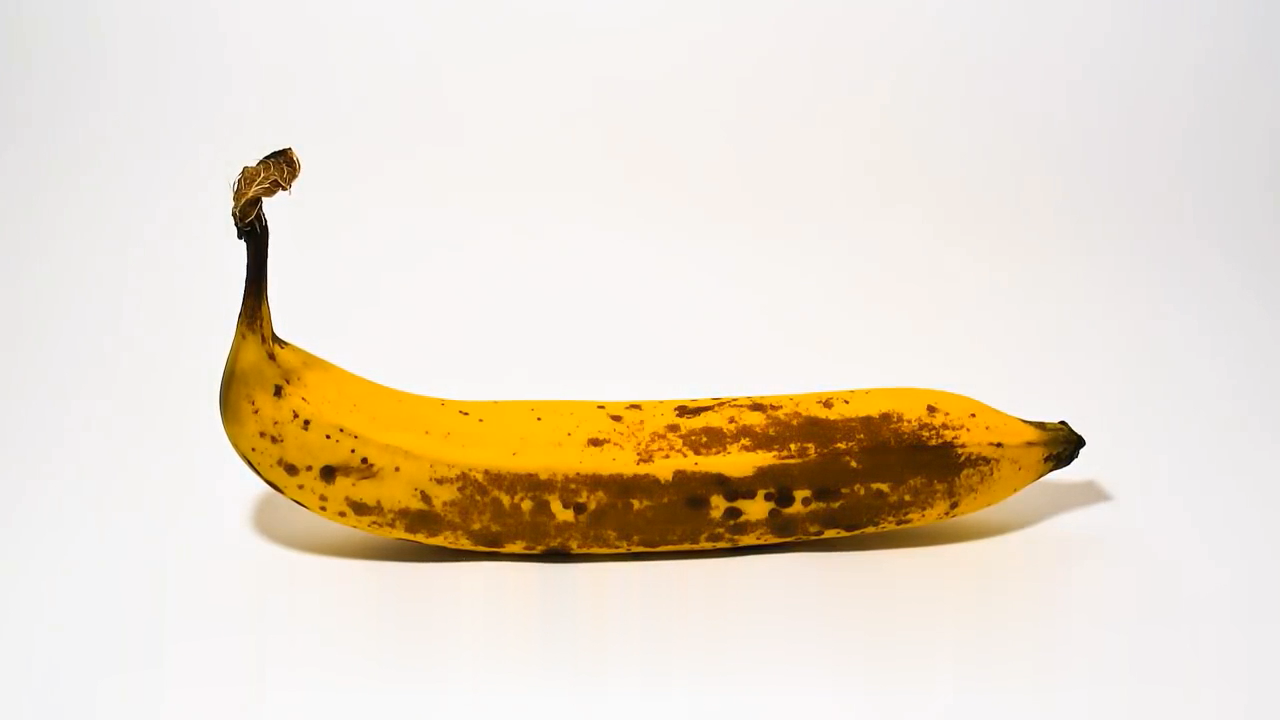
\includegraphics[width=12cm]{dataset_exemplo/banana/banana_016.png}};
  \draw[blue, very thick]
    plot[smooth cycle] coordinates {
      (1.55,2.25) (2.05,4.35) (2.75,4.95) (3.35,4.35)
      (3.85,3.55) (5.6,3.5) (8.25,3.35) (10.15,2.85)
      (10.55,2.42) (9.45,1.82) (6.25,1.52) (3.05,1.55)
      (1.65,1.82)
    };
  \node[blue, fill=white, inner sep=2pt] at (8.65,4.05)
    {máscara aproximada da fruta};
  \draw[blue, ->, thick] (7.9,3.8) -- (7.1,3.28);

  \draw[red, very thick] (4.69,2.34) rectangle (5.44,2.58);
  \node[red, fill=white, inner sep=2pt] at (3.75,3.35)
    {RI pequena interna};
  \draw[red, ->, thick] (4.35,3.12) -- (5.06,2.58);
\end{tikzpicture}
\caption{Exemplo real de duas formas de região de interesse em uma imagem do dataset: uma RI pequena no interior da banana e uma máscara aproximada da fruta inteira.}
\label{fig:ri-banana}
\end{figure}

A RI pequena indicada na Figura~\ref{fig:ri-banana} se aproxima da estratégia usada no trabalho de Valesan (2022), disponível no repositório em \path{referencias/dispositivocontrolematuracao.pdf}, em que recortes internos eram escolhidos em regiões de cor aproximadamente uniforme. Essa abordagem reduz a influência do fundo e evita partes da fruta com sombra, brilho ou borda, mas mede apenas uma pequena região. A Figura~\ref{fig:recortes-ri-banana} mostra os recortes reais dessa RI ao longo das 32 imagens da sequência.

\begin{figure}[H]
\centering
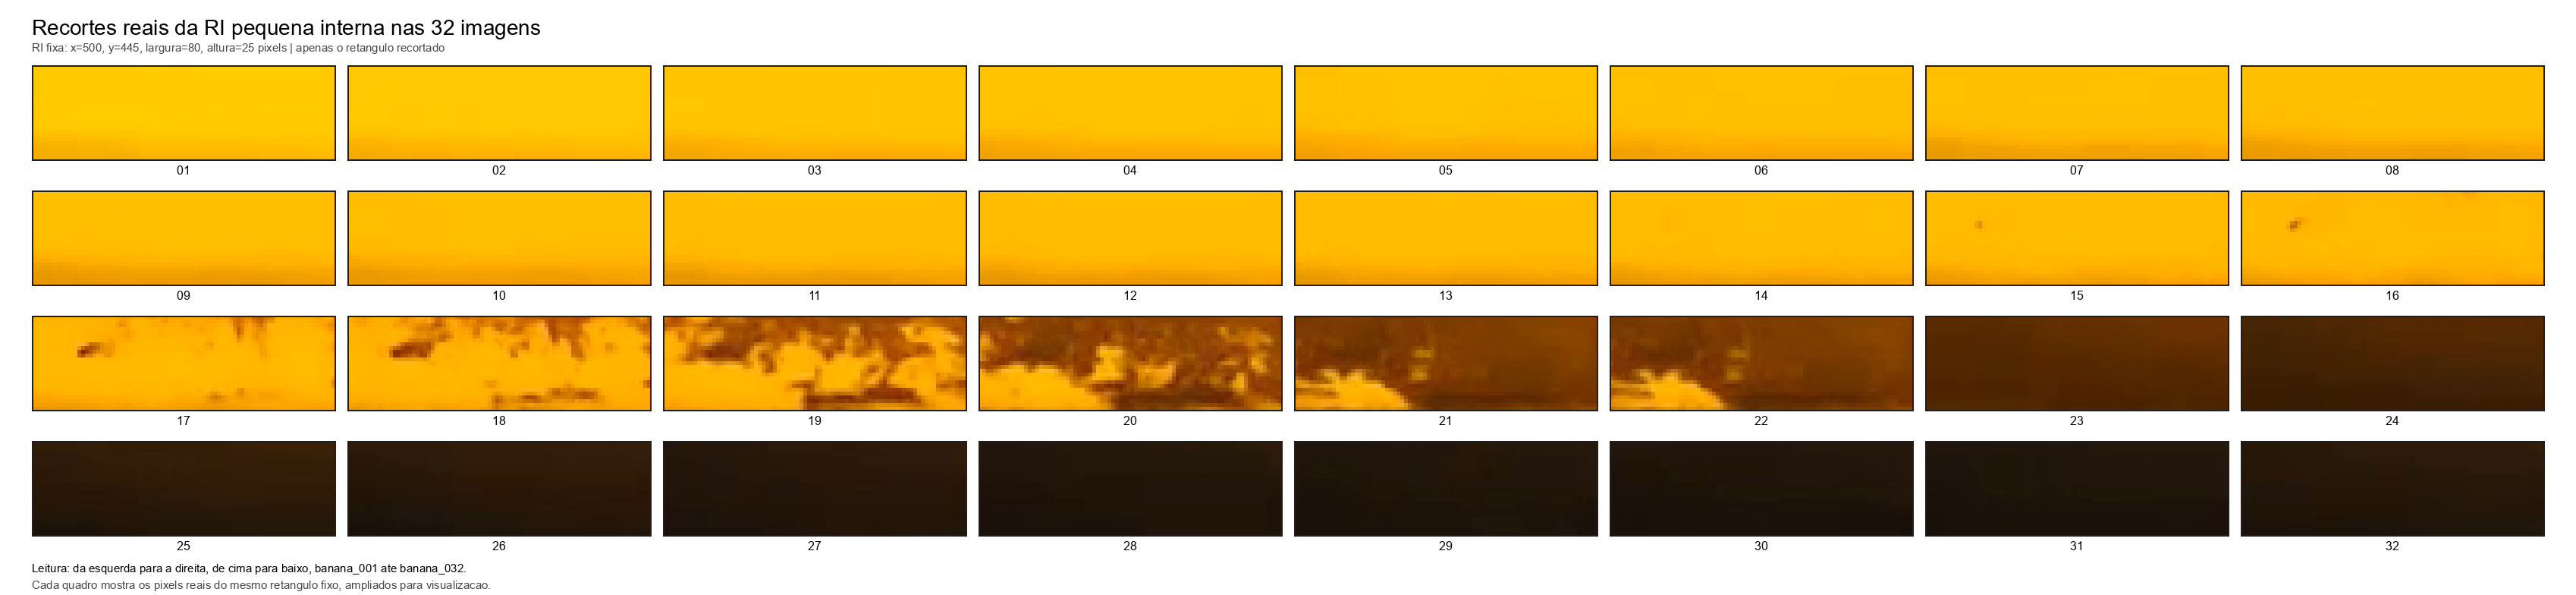
\includegraphics[width=\linewidth]{matriz_recortes_ri_banana_v2.png}
\caption{Recortes reais da RI pequena interna nas 32 imagens de banana. Cada quadro mostra apenas o retângulo selecionado na imagem correspondente, ampliado para visualização.}
\label{fig:recortes-ri-banana}
\end{figure}

A máscara aproximada da fruta inteira, também mostrada na Figura~\ref{fig:ri-banana}, é mais parecida com a estratégia simplificada usada no script desta aula: em vez de escolher manualmente um quadrado, o programa tenta descartar pixels quase brancos e calcula a média dos demais pixels. Essa abordagem usa mais informação da imagem, mas pode incluir sombras, bordas, manchas e trechos de fundo que não foram removidos perfeitamente. O Quadro~\ref{qua:comparacao-ri} resume a diferença numérica entre as duas escolhas para a Figura~\ref{fig:ri-banana}.

\refstepcounter{quadro}\label{qua:comparacao-ri}
\begin{cmdbox}[Quadro~\thequadro{} -- Comparação entre duas escolhas de RI na Figura~\ref{fig:ri-banana}]
\begin{tabularx}{\linewidth}{@{}C C C C >{\raggedright\arraybackslash}X@{}}
\toprule
\textbf{Região analisada} & \textbf{R} & \textbf{G} & \textbf{B} & \textbf{Comentário} \\
\midrule
RI pequena interna & 253,88 & 181,29 & 0,04 & Mede uma região amarela local, sem fundo aparente no recorte escolhido. \\
Máscara aproximada & 179,62 & 126,26 & 35,47 & Usa muito mais pixels da fruta; inclui manchas, bordas e sombras. \\
\bottomrule
\end{tabularx}
\end{cmdbox}

Os valores apresentados no Quadro~\ref{qua:comparacao-ri} são diferentes porque as perguntas de medição também são diferentes. A RI pequena responde: ``qual é a cor média desta região específica da banana?''. A máscara aproximada responde: ``qual é a média dos pixels que o algoritmo considerou como não fundo?''. Em uma análise real, a escolha da RI deve ser definida antes do experimento e mantida constante para todas as imagens.

O script da atividade usa a máscara aproximada por padrão. Para explorar uma RI retangular fixa, existe a opção \texttt{--roi}. O Quadro~\ref{qua:comando-roi} usa uma RI de largura 80 pixels e altura 25 pixels, começando na posição \texttt{x=500} e \texttt{y=445} da imagem:

\refstepcounter{quadro}\label{qua:comando-roi}
\begin{codebox}[Quadro~\thequadro{} -- Comando para processar uma RI retangular fixa]
python 003_material_de_apoio/scripts/analise_rgb.py \
003_material_de_apoio/dataset_exemplo/banana \
--roi 500 445 80 25 \
--csv banana_roi.csv --grafico banana_roi.png
\end{codebox}

Essa RI fixa é útil para discutir o método, mas deve ser usada com cuidado: se a fruta mudar de posição, o retângulo pode deixar de apontar para a mesma região física da fruta.

A Figura~\ref{fig:comparacao-ri-mascara} compara os gráficos produzidos pelas duas estratégias ao longo das 32 imagens de banana. A máscara aproximada da fruta inteira tende a produzir curvas mais suaves do que a RI pequena, pois usa muitos pixels da fruta. Mesmo assim, quando o fundo é removido de forma mais adequada, as curvas passam a refletir melhor as mudanças visuais da banana. A RI pequena é mais sensível ao ponto escolhido: ela pode destacar melhor uma região local da polpa, mas também pode variar bastante se a fruta mudar de posição, se a mancha passar pela região escolhida ou se o retângulo pegar sombra.

\begin{figure}[H]
\centering
\begin{minipage}{0.48\linewidth}
\centering
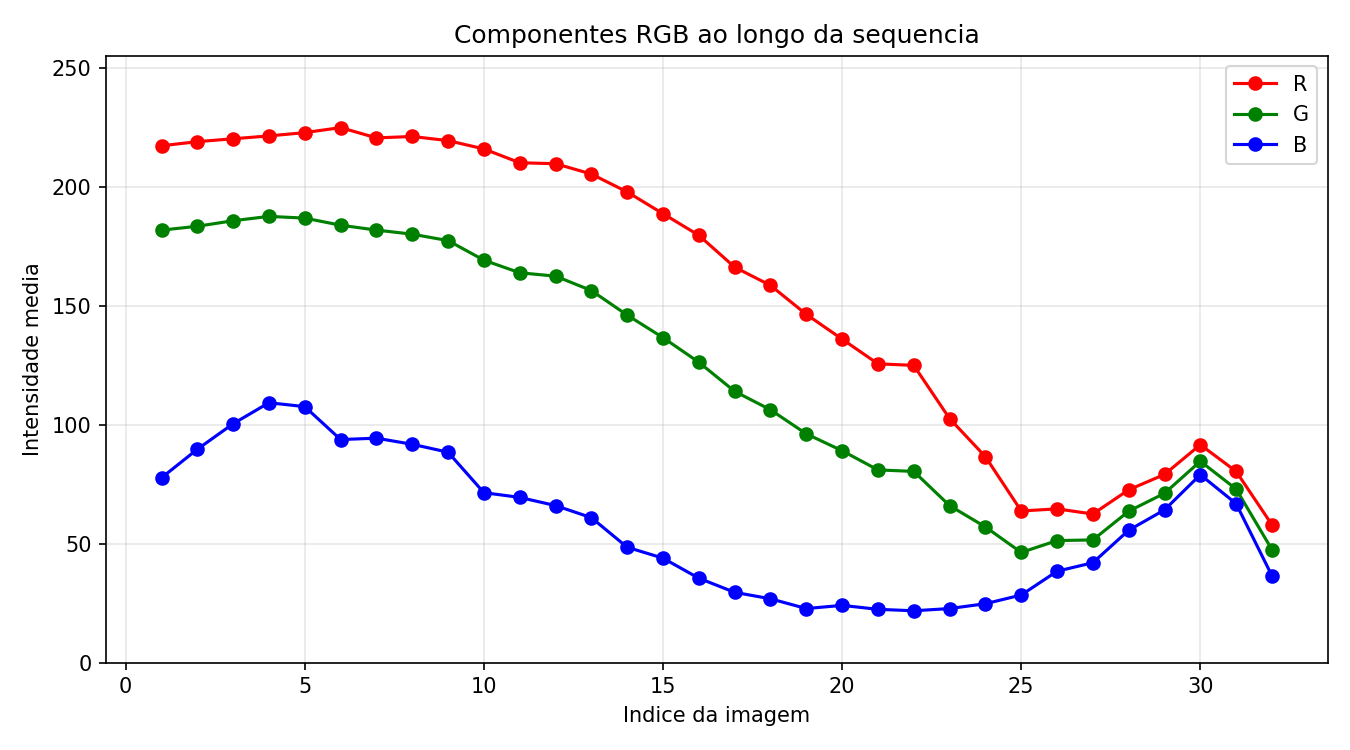
\includegraphics[width=\linewidth]{grafico_exemplo_banana.png}
\small Máscara aproximada da fruta
\end{minipage}
\hfill
\begin{minipage}{0.48\linewidth}
\centering
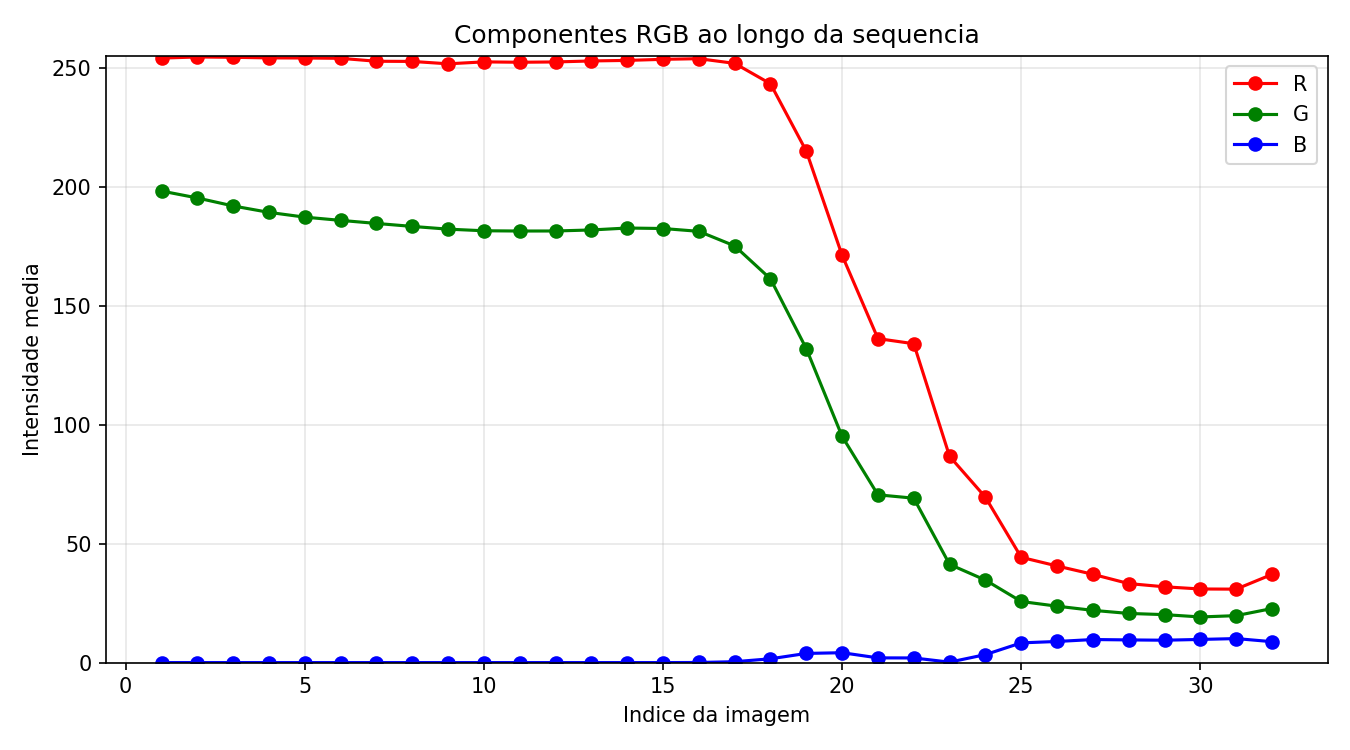
\includegraphics[width=\linewidth]{banana_roi.png}
\small RI pequena interna
\end{minipage}
\caption{Comparação entre o processamento usando uma máscara aproximada da fruta inteira e uma RI pequena interna.}
\label{fig:comparacao-ri-mascara}
\end{figure}

\subsection{Por que ignorar o fundo branco?}

Muitas imagens usadas na atividade possuem fundo quase branco. Se a média RGB for calculada usando todos os pixels da imagem, o resultado pode representar mais o fundo do que a fruta. Isso é um problema experimental importante: nem todo pixel da imagem pertence ao objeto de interesse.

Para reduzir esse efeito, o script ignora pixels quase brancos. A regra usada é simples:

\begin{codebox}
R >= 220, G >= 220 e B >= 220
\end{codebox}

Quando isso ocorre, o pixel é considerado fundo e não entra no cálculo da média.

Essa técnica é uma forma simples de limiarização, também chamada de \textit{thresholding}. A limiarização é uma técnica clássica de segmentação em processamento de imagens: uma regra separa pixels em classes, por exemplo ``fundo'' e ``objeto'', usando um ou mais valores de corte. Um método muito conhecido para escolher limiares automaticamente é o método de Otsu, que busca separar classes a partir do histograma de intensidades (OTSU, 1979). Livros de processamento de imagens, como Gonzalez e Woods (2018), também tratam a limiarização como uma técnica básica de segmentação.

A Figura~\ref{fig:pixels-desconsiderados} mostra o efeito da regra usada no script sobre a imagem \texttt{banana\_016.png}. Os pixels pretos são aqueles que foram descartados por serem considerados fundo quase branco. Os demais pixels foram mantidos no cálculo.

\begin{figure}[H]
\centering
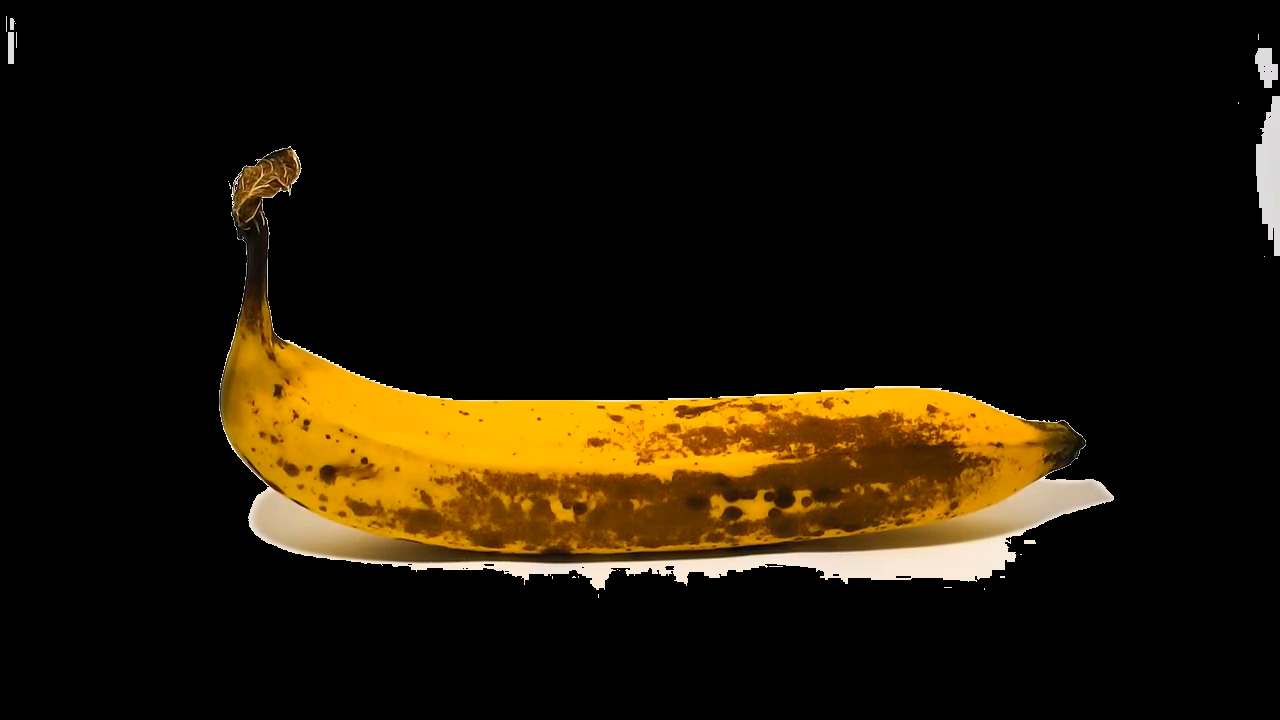
\includegraphics[width=0.9\linewidth]{banana_016_pixels_desconsiderados.png}
\caption{Imagem de diagnóstico: pixels em preto foram desconsiderados pela regra \texttt{R >= 220, G >= 220 e B >= 220}; os demais pixels foram mantidos no cálculo.}
\label{fig:pixels-desconsiderados}
\end{figure}

Na Figura~\ref{fig:pixels-desconsiderados}, quase todo o fundo branco fica preto. Isso indica que a maior parte do fundo foi descartada antes do cálculo da média. Na imagem analisada, o limiar 220 descartou cerca de 83\% dos pixels. Se fosse usado um limiar mais alto, como 245, apenas cerca de 12\% dos pixels seriam removidos; muitos pixels de fundo ainda entrariam na média. Esse fundo residual puxaria os valores RGB para perto do branco e faria as curvas variarem pouco, escondendo parte das mudanças visuais da banana.

Escolher o limiar é uma decisão experimental. Um limiar alto, como 245, só remove pixels muito brancos. Um limiar mais baixo, como 220, remove uma parte maior do fundo, mas pode começar a remover regiões claras do objeto, dependendo da cor da fruta e da iluminação. Por isso, o limiar deve ser escolhido observando imagens de teste, avaliando a imagem segmentada e mantendo a mesma regra para todas as imagens que serão comparadas.

O script para análise de imagens presente neste material permite testar outros valores com a opção \texttt{--limite-branco}. A Seção~\ref{subsec:teste-limiar} apresenta um comando específico para repetir o processamento usando outro limiar.

Essa técnica não é perfeita. Ela pode falhar se o fundo não for branco, se a fruta possuir regiões muito claras ou se houver sombras fortes. Mesmo assim, é suficiente para mostrar uma ideia central: antes de medir, é necessário decidir qual região da imagem representa o objeto de interesse.

\section{Dataset usado na atividade}

As imagens desta atividade foram retiradas do FruitQ, um dataset público disponível no Kaggle para estudo de qualidade visual de frutas e hortaliças. O dataset completo é bem maior do que o material usado nesta aula e contém diferentes produtos, como banana, pepino, uva, caqui, mamão, pêssego, pera, pimentão, morango, tomate e melancia. As imagens são organizadas em classes visuais de qualidade, como boa, intermediária e deteriorada, dependendo da fruta.

Como o objetivo da aula não é treinar um classificador nem trabalhar com um banco de imagens grande, foi preparado um subconjunto didático pequeno. Isso reduz o tempo de processamento, facilita a visualização dos resultados e evita que a organização dos arquivos se torne o foco da atividade.

Neste material, foram usadas duas frutas:

\begin{itemize}
  \item banana, usada no exemplo guiado;
  \item tomate, usado na atividade dos alunos.
\end{itemize}

Cada conjunto possui 32 imagens. O dataset completo não foi mantido neste repositório, pois é grande para a atividade. Ele pode ser acessado diretamente no Kaggle em \url{https://www.kaggle.com/datasets/sholzz/fruitq-dataset}. Para a aula, os arquivos foram copiados para \texttt{003\_material\_de\_apoio} e renomeados com um padrão simples:

\begin{codebox}
banana_001.png
banana_002.png
...
banana_032.png
\end{codebox}

e

\begin{codebox}
tomate_001.png
tomate_002.png
...
tomate_032.png
\end{codebox}

Esse tipo de nomenclatura é parecido com o que se espera em uma coleta real automatizada: todos os arquivos seguem o mesmo formato, mudando apenas o número da imagem.

\subsection{Ordem das imagens}

As imagens foram selecionadas respeitando a ordem numérica original do dataset e espaçadas de forma uniforme dentro de cada etapa. No conjunto didático, a sequência foi organizada conforme o Quadro~\ref{qua:etapas-sequencia}:

\refstepcounter{quadro}\label{qua:etapas-sequencia}
\begin{cmdbox}[Quadro~\thequadro{} -- Etapas da sequência]
\begin{tabularx}{\linewidth}{@{}C C >{\raggedright\arraybackslash}X@{}}
\toprule
\textbf{Índices} & \textbf{Etapa} & \textbf{Interpretação} \\
\midrule
1 a 11 & boa & Fruta em melhor condição visual. \\
12 a 21 & intermediária & Fruta com sinais intermediários de alteração. \\
22 a 32 & deteriorada & Fruta com deterioração mais evidente. \\
\bottomrule
\end{tabularx}
\end{cmdbox}

A sequência não deve ser tratada como uma medição temporal real de laboratório. Ela representa uma ordem visual de alteração, útil para praticar processamento de imagem.

\section{Controle experimental e fontes de erro}

Em um experimento real, não basta escolher um algoritmo. A forma de captura influencia diretamente os resultados. No estudo usado como referência, as imagens eram adquiridas periodicamente em uma câmara com ambiente controlado, junto com outras grandezas, como temperatura, umidade, luminosidade, dióxido de carbono e massa dos frutos. O trabalho de Valesan está disponível neste repositório em \path{referencias/dispositivocontrolematuracao.pdf}.

Esse cuidado é importante porque a cor medida pela câmera pode mudar por motivos que não estão relacionados à maturação:

\begin{itemize}
  \item variação da iluminação;
  \item sombras;
  \item mudança de posição da câmera;
  \item mudança de posição da fruta;
  \item ajuste automático da câmera;
  \item reflexos e brilho na superfície.
\end{itemize}

Por isso, técnicas como uso de fundo de referência, normalização, escolha de regiões de interesse e média móvel podem ser usadas para reduzir variações indesejadas. Nesta aula, aplicaremos apenas uma primeira aproximação: remover pixels de fundo quase branco e observar as médias RGB.

\subsection{Relação com a atividade prática}

O trabalho de referência acompanhava frutos ao longo do tempo real, com imagens capturadas periodicamente. No nosso caso, usaremos o subconjunto didático do FruitQ apresentado na seção anterior. A sequência foi organizada para representar uma progressão visual de qualidade, e não uma coleta temporal real.

Mesmo assim, o raciocínio experimental é o mesmo:

\begin{codebox}
imagem -> região analisada -> valores RGB
       -> tabela -> gráfico -> interpretação
\end{codebox}

A atividade é, portanto, uma versão reduzida do processo usado em estudos de maturação por imagem. O objetivo é entender a lógica da medição antes de avançar para técnicas mais complexas.

\section{Execução do script}

O aluno não precisa escrever o programa em Python do zero. O script já está pronto. A tarefa é executar o comando, conferir os arquivos gerados e interpretar o resultado.

O script está localizado em:

\begin{codebox}
003_material_de_apoio/scripts/analise_rgb.py
\end{codebox}

As bibliotecas necessárias estão listadas em:

\begin{codebox}
003_material_de_apoio/requirements.txt
\end{codebox}

No computador Windows do laboratório, se for necessário instalar as bibliotecas, abra o PowerShell na pasta do material e use o comando do Quadro~\ref{qua:comando-instalar-bibliotecas}:

\refstepcounter{quadro}\label{qua:comando-instalar-bibliotecas}
\begin{codebox}[Quadro~\thequadro{} -- Comando para instalar as bibliotecas]
python -m pip install -r 003_material_de_apoio/requirements.txt
\end{codebox}

Antes de executar o script, também é possível conferir se o Python está disponível com o comando do Quadro~\ref{qua:comando-versao-python}:

\refstepcounter{quadro}\label{qua:comando-versao-python}
\begin{codebox}[Quadro~\thequadro{} -- Comando para verificar a versão do Python]
python --version
\end{codebox}

\subsection{Exemplo com banana}

Para processar o conjunto de banana, execute o comando do Quadro~\ref{qua:comando-banana}:

\refstepcounter{quadro}\label{qua:comando-banana}
\begin{codebox}[Quadro~\thequadro{} -- Comando para processar o exemplo com banana]
python 003_material_de_apoio/scripts/analise_rgb.py \
003_material_de_apoio/dataset_exemplo/banana
\end{codebox}

O comando gera dois arquivos:

\begin{codebox}
resultado_rgb.csv
grafico_rgb.png
\end{codebox}

O CSV é uma tabela com uma linha por imagem. O gráfico mostra como os canais R, G e B variam ao longo da sequência.

\subsection{Teste com outro limiar de fundo}
\label{subsec:teste-limiar}

Depois de processar o exemplo com o valor padrão, é possível repetir a análise mudando o limiar de fundo. O comando do Quadro~\ref{qua:comando-limiar} usa o valor 245 para comparar o resultado com o processamento padrão:

\refstepcounter{quadro}\label{qua:comando-limiar}
\begin{codebox}[Quadro~\thequadro{} -- Comando para testar outro limiar de fundo]
python 003_material_de_apoio/scripts/analise_rgb.py \
003_material_de_apoio/dataset_exemplo/banana \
--limite-branco 245 \
--csv banana_limiar245.csv --grafico banana_limiar245.png
\end{codebox}

\subsection{Atividade com tomate}

Depois do exemplo, os alunos devem repetir o processamento com o conjunto de tomate usando o comando do Quadro~\ref{qua:comando-tomate}:

\refstepcounter{quadro}\label{qua:comando-tomate}
\begin{codebox}[Quadro~\thequadro{} -- Comando para processar a atividade com tomate]
python 003_material_de_apoio/scripts/analise_rgb.py \
003_material_de_apoio/dataset_atividade/tomate \
--csv tomate_rgb.csv --grafico tomate_rgb.png
\end{codebox}

O uso de \texttt{--csv} e \texttt{--grafico} permite escolher os nomes dos arquivos de saída.

\section{Entendendo o script Python}

O script \texttt{analise\_rgb.py} foi organizado em funções pequenas. Isso facilita a leitura: cada função tem uma responsabilidade específica. O aluno não precisa memorizar todos os comandos, mas deve entender o caminho geral dos dados dentro do programa.

\subsection{Bibliotecas usadas}

No início do script aparecem as importações:

\begin{codebox}
from argparse import ArgumentParser
from csv import DictWriter
from pathlib import Path
from PIL import Image
\end{codebox}

Cada biblioteca tem uma função:

\begin{cmdbox}[Bibliotecas do script]
\begin{tabularx}{\linewidth}{@{}C >{\raggedright\arraybackslash}X@{}}
\toprule
\textbf{Biblioteca} & \textbf{Uso no script} \\
\midrule
argparse & Ler opções digitadas no terminal, como \texttt{--csv} e \texttt{--grafico}. \\
csv & Salvar os resultados em uma tabela CSV. \\
pathlib & Trabalhar com caminhos de arquivos e pastas. \\
PIL & Abrir imagens e acessar os pixels. \\
matplotlib & Gerar o gráfico RGB. \\
\bottomrule
\end{tabularx}
\end{cmdbox}

\subsection{Listagem das imagens}

A função \texttt{listar\_imagens} recebe uma pasta e retorna os arquivos de imagem encontrados nela:

\begin{codebox}
def listar_imagens(pasta):
    extensoes = {".jpg", ".jpeg", ".png"}
    imagens = []
    for arquivo in Path(pasta).iterdir():
        if arquivo.suffix.lower() in extensoes:
            imagens.append(arquivo)
    return sorted(imagens)
\end{codebox}

O conjunto \texttt{extensoes} define quais formatos serão aceitos. O comando \texttt{iterdir()} percorre os arquivos da pasta. O \texttt{sorted} coloca os nomes em ordem. Como os arquivos foram padronizados como \texttt{banana\_001.png}, \texttt{banana\_002.png} e assim por diante, essa ordenação fica coerente com a sequência da atividade.

\subsection{Identificação da etapa}

Como os arquivos seguem uma sequência didática, a função \texttt{etapa\_por\_indice} associa cada intervalo de imagens a uma etapa:

\begin{codebox}
def etapa_por_indice(indice):
    if indice <= 11:
        return "boa"
    if indice <= 21:
        return "intermediaria"
    return "deteriorada"
\end{codebox}

Assim, as imagens 1 a 11 são tratadas como boas, as imagens 12 a 21 como intermediárias, e as imagens 22 a 32 como deterioradas. Essa informação aparece depois na coluna \texttt{etapa} do CSV.

\subsection{Abertura da imagem}

A função mais importante é \texttt{media\_rgb}. Ela começa abrindo a imagem:

\begin{codebox}
imagem = Image.open(caminho).convert("RGB")
if roi:
    x, y, largura, altura = roi
    imagem = imagem.crop((x, y, x + largura, y + altura))
imagem.thumbnail((tamanho_maximo, tamanho_maximo))
\end{codebox}

O comando \texttt{Image.open} abre o arquivo. O \texttt{convert("RGB")} garante que a imagem será analisada com três canais de cor. Se o usuário informar \texttt{--roi}, o comando \texttt{crop} recorta uma região retangular antes do cálculo. O \texttt{thumbnail} reduz imagens muito grandes para acelerar o processamento, mantendo a proporção original.

\subsection{Percorrendo os pixels}

Depois, o script inicia acumuladores:

\begin{codebox}
soma_r = 0
soma_g = 0
soma_b = 0
contador = 0
\end{codebox}

Essas variáveis guardam a soma dos valores R, G e B e a quantidade de pixels usados. Em seguida, o programa percorre os pixels:

\begin{codebox}
for r, g, b in imagem.getdata():
    ...
\end{codebox}

Em cada repetição, \texttt{r}, \texttt{g} e \texttt{b} recebem os valores de um pixel.

\subsection{Remoção simples do fundo}

O script verifica se o pixel é quase branco:

\begin{codebox}
fundo_branco = (
    r >= limite_branco and
    g >= limite_branco and
    b >= limite_branco
)
if ignorar_fundo and fundo_branco:
    continue
\end{codebox}

O valor padrão de \texttt{limite\_branco} é 220. Se os três canais forem maiores ou iguais a esse valor, o pixel é considerado fundo. O comando \texttt{continue} pula esse pixel, ou seja, ele não entra na média.

Se o usuário executar o script com \texttt{--imagem-inteira}, a variável \texttt{ignorar\_fundo} fica falsa e o programa usa todos os pixels, inclusive o fundo.

Se o usuário informar \texttt{--limite-branco}, o valor padrão 220 é substituído pelo valor escolhido. Isso permite testar limiares mais rígidos ou mais permissivos sem editar o código.

\subsection{Cálculo das médias}

Os pixels aceitos são somados:

\begin{codebox}
soma_r += r
soma_g += g
soma_b += b
contador += 1
\end{codebox}

No final, a função retorna as médias:

\begin{codebox}
media_r = soma_r / contador
media_g = soma_g / contador
media_b = soma_b / contador
return media_r, media_g, media_b, contador
\end{codebox}

Isso produz quatro informações: média de vermelho, média de verde, média de azul e quantidade de pixels usados.

\subsection{Salvando o CSV}

A função \texttt{salvar\_csv} cria uma tabela com os resultados:

\begin{codebox}
campos = ["indice", "arquivo", "etapa",
          "media_r", "media_g", "media_b", "pixels_usados"]
\end{codebox}

Cada imagem processada vira uma linha no CSV. Esse arquivo é importante porque permite analisar os dados depois em uma planilha, em outro programa Python ou em relatórios.

\subsection{Gerando o gráfico}

A função \texttt{salvar\_grafico} separa os dados em listas:

\begin{codebox}
x = [linha["indice"] for linha in linhas]
r = [linha["media_r"] for linha in linhas]
g = [linha["media_g"] for linha in linhas]
b = [linha["media_b"] for linha in linhas]
\end{codebox}

Depois, gera três curvas:

\begin{codebox}
plt.plot(x, r, "r-o", label="R")
plt.plot(x, g, "g-o", label="G")
plt.plot(x, b, "b-o", label="B")
\end{codebox}

As letras \texttt{r}, \texttt{g} e \texttt{b} definem as cores das linhas no gráfico: vermelho, verde e azul.

\subsection{Fluxo principal}

A função \texttt{main} reúne todas as etapas:

\begin{enumerate}
  \item lê os argumentos digitados no terminal;
  \item encontra as imagens na pasta informada;
  \item processa uma imagem por vez;
  \item monta uma lista de resultados;
  \item salva o CSV;
  \item salva o gráfico;
  \item mostra mensagens finais no terminal.
\end{enumerate}

O trecho final:

\begin{codebox}
if __name__ == "__main__":
    main()
\end{codebox}

significa que a função \texttt{main} será executada quando o arquivo for chamado diretamente pelo terminal.

\subsection{Resumo do caminho dos dados}

O fluxo completo do script pode ser resumido assim:

\begin{codebox}
pasta de imagens
      -> lista de arquivos
      -> leitura de cada imagem
      -> pixels RGB
      -> remoção do fundo quase branco
      -> média R, G e B
      -> CSV e gráfico
\end{codebox}

\section{Como interpretar a tabela}

O arquivo CSV possui as seguintes colunas:

\begin{cmdbox}[Colunas do CSV]
\begin{tabularx}{\linewidth}{@{}C >{\raggedright\arraybackslash}X@{}}
\toprule
\textbf{Coluna} & \textbf{Significado} \\
\midrule
indice & Ordem da imagem na sequência. \\
arquivo & Nome do arquivo processado. \\
etapa & Etapa didática: boa, intermediária ou deteriorada. \\
media\_r & Média do canal vermelho. \\
media\_g & Média do canal verde. \\
media\_b & Média do canal azul. \\
pixels\_usados & Quantidade de pixels considerados após remover o fundo quase branco. \\
\bottomrule
\end{tabularx}
\end{cmdbox}

Para visualizar as primeiras linhas da tabela no terminal, use o comando do Quadro~\ref{qua:comando-ver-csv}:

\refstepcounter{quadro}\label{qua:comando-ver-csv}
\begin{codebox}[Quadro~\thequadro{} -- Comando para visualizar as primeiras linhas do CSV]
Get-Content resultado_rgb.csv -TotalCount 10
\end{codebox}

\section{Como interpretar o gráfico}

O gráfico apresenta três curvas: uma para o canal R, uma para o canal G e uma para o canal B. O eixo horizontal representa a ordem das imagens. O eixo vertical representa a intensidade média de cada canal.

\begin{figure}[H]
\centering
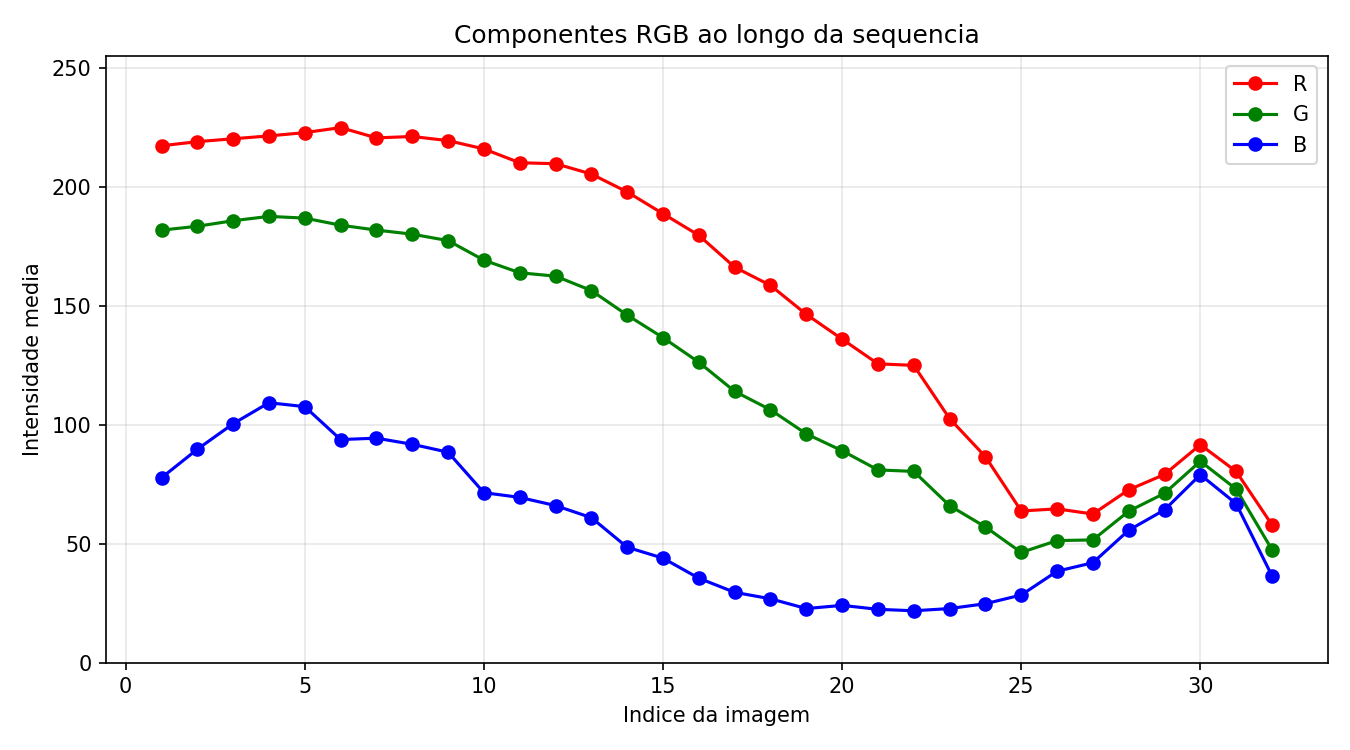
\includegraphics[width=0.9\linewidth]{grafico_exemplo_banana.png}
\caption{Exemplo de gráfico RGB gerado para a sequência de banana.}
\label{fig:grafico-banana}
\end{figure}

Durante a interpretação do gráfico, como no exemplo da Figura~\ref{fig:grafico-banana}, observe:

\begin{itemize}
  \item qual canal varia mais;
  \item se a mudança é gradual ou abrupta;
  \item se há diferença entre as etapas boa, intermediária e deteriorada;
  \item se algum ponto parece fora do padrão;
  \item se o fundo, a sombra ou a iluminação podem ter influenciado o resultado.
\end{itemize}

\section{Limitações do método}

O cálculo da média RGB é simples e fácil de entender, mas possui limitações. Ele resume a imagem inteira em apenas três números. Com isso, detalhes importantes podem ser perdidos.

Alguns fatores que podem afetar o resultado são:

\begin{itemize}
  \item iluminação diferente entre imagens;
  \item sombras;
  \item mudança de posição da fruta;
  \item tamanho aparente do objeto;
  \item fundo da imagem;
  \item presença de mais de uma fruta na mesma imagem.
\end{itemize}

Essas limitações são parte importante da discussão. Em metrologia por imagem, medir não é apenas aplicar um algoritmo; é também controlar as condições de captura e entender as fontes de erro.

\section{Relação com os módulos anteriores}

Nos módulos 1 e 2, a captura de imagens foi discutida com comandos de terminal, scripts e automação em um sistema embarcado. Esses elementos fazem parte da etapa de aquisição dos dados.

Neste módulo, a análise RGB representa uma etapa posterior do pipeline:

\begin{codebox}
experimento -> captura -> armazenamento -> processamento -> gráfico
\end{codebox}

Uma captura automatizada ajuda a produzir imagens mais comparáveis, porque reduz variações de horário, procedimento e intervenção manual. O processamento em Python transforma essas imagens em números que podem ser analisados e discutidos.

\section{Questões para discussão}

\begin{enumerate}
  \item Qual canal RGB mudou mais ao longo da sequência?
  \item A mudança entre as etapas parece gradual?
  \item A média RGB separa bem as imagens boas, intermediárias e deterioradas?
  \item O que mudaria se o fundo branco fosse incluído no cálculo?
  \item Que melhoria poderia tornar a medição mais confiável?
\end{enumerate}

\section{Referência de apoio}

GONZALEZ, Rafael C.; WOODS, Richard E. \textit{Digital Image Processing}. 4. ed. New York: Pearson, 2018.

OTSU, Nobuyuki. A threshold selection method from gray-level histograms. \textit{IEEE Transactions on Systems, Man, and Cybernetics}, v. 9, n. 1, p. 62--66, 1979.

SHOLZZ. \textit{FruitQ Dataset}. Kaggle. Disponível em: \url{https://www.kaggle.com/datasets/sholzz/fruitq-dataset}.

VALESAN, Dyorgyo Pompermaier. \textit{Dispositivo para controle de maturação de frutas e controle de eficiência de biofilmes comestíveis}. Trabalho de Conclusão de Curso (Bacharelado em Engenharia Eletrônica) -- Universidade Tecnológica Federal do Paraná, Toledo, 2022. Arquivo disponível neste repositório em \path{referencias/dispositivocontrolematuracao.pdf}.

\end{document}
